%%%%             %%%%
%%%% ADICIONAL 2 %%%%
%%%%             %%%%

\chapter{Material adicional}
\label{chap:material-adicional}

\section{Textract y Document AI}
\label{sec:textract-y-document-ai}

Dos servicios diferentes a los productos mencionados en el Capítulo \ref{chap:estado-arte}, pero en un ámbito relacionado con el problema son, Textract de Amazon \cite{solucionesComerciales_amazon_textract} y Document AI de Google \cite{solucionesComerciales_google_documentAI}. Ninguno de los dos soporta el flujo de información explicado, ni están pensados para ser solución para el usuario final. Lo que ofrecen es un \emph{\acrshort{api}} capaz de recibir documentos y generar información estructurada como salida. El caso de Textract es totalmente opaco y por tanto no configurable. La salida consiste en ficheros JSON donde puede haber varios tipos de objetos: páginas, líneas y palabras, información de formularios (en formato par clave-valor), tablas, y elementos seleccionables, como casillas. Además es capaz de identificar notas manuscritas. El servicio de Google permite definir \emph{processors}, que son plantillas específicas para modelos de documentos conocidos. Parece que el servicio es muy reciente y la mayor parte de las funcionalidades publicitadas están en una beta cerrada. Cualquiera de ellos podría utilizarse como parte de una solución más completa. Como otros servicios en la nube, se paga según la cantidad de uso que se hace del servicio o lo que es lo mismo, la carga de trabajo procesada.

\section{Manual de usuario}
\label{sec:instalacion-software}

Se explica seguidamente como proceder a la instalación del software así como realizar la ejecución manual de un conjunto de documentos.

\subsection{Instalación del software}

La instalación completa desde el código fuente implica la descarga del contenido presente en el repositorio git.

En esta sección se asume que se utilizará una distribución Ubuntu 18.04 igual a la empleada durante el desarrollo. Para la correcta compilación y ejecución, es necesario que varias aplicaciones y librerías estén disponibles en el sistema. En el caso de las nuevas versiones de Ubuntu, la lista de paquetes a instalar no presentará diferencias, pero si se utiliza Fedora u otras distribuciones, será necesario averiguar qué paquetes contienen el software utilizado e instalarlos.

Se pueden distinguir dos escenarios distintos. Los requisitos necesarios para compilar los ficheros fuente y aquellos imprescindibles únicamente para ejecutar la aplicación. Para el primer caso se debe utilizar el comando mostrado en \ref{lst:requisitos-para-compilacion}. El paquete \verb|build-essential| instala la mayor parte de las aplicaciones, como el compilador de C y Make.

\begin{lstlisting}[language=bash,caption={Dependencias para la compilación},label=lst:requisitos-para-compilacion]
sudo apt-get build-essential libpcre2-dev bison flex
\end{lstlisting}

En el caso de tener ya la aplicación compilada y empaquetada, será necesarios instalar los componentes para la ejecución, como Tesseract, el software de OCR. La orden del listado \ref{lst:requisitos-para-ejecucion} instalará estos requisitos.

\begin{lstlisting}[language=bash,caption={Dependencias para la ejecución},label=lst:requisitos-para-ejecucion]
sudo apt-get install unzip poppler-utils mediainfo tesseract-ocr tesseract-ocr-spa jq python3-opencv jq bc
\end{lstlisting}

De manera opcional pero recomendable, se puede utilizar un PPA específico para obtener una versión actualizada de Tesseract. Un PPA en el entorno Ubuntu, es un repositorio personal de paquetes listos para su instalación, en este caso mantenido por Alexander Pozdnyakov \footnote{\url{https://launchpad.net/~alex-p/+archive/ubuntu/tesseract-ocr}}. La activación de este repositorio debe hacerse previamente a la instalación del software. Es necesario ejecutar los comandos del listado \ref{lst:activar-ppa-tesseract}.

\begin{lstlisting}[language=bash,caption={Activar PPA de Tesseract},label=lst:activar-ppa-tesseract]
sudo add-apt-repository ppa:alex-p/tesseract-ocr
sudo apt-get update
\end{lstlisting}

\subsection{Ejecución manual}

Para una correcta ejecución totalmente manual, es necesario primero inicializar algunos parámetros de configuración. Se procederá primero leyendo el fichero de configuración que define todas las rutas utilizadas por el \emph{engine}. Así mismo se creará el directorio para los ficheros de entrada:

\begin{lstlisting}[language=bash,caption={},label={}]
conf_file='conf/engine-dev.sh'
source $conf_file
mkdir -p $input_dir
\end{lstlisting}

Acto seguido ya se puede obtener el identificador para un nuevo trabajo:

\begin{lstlisting}[language=bash,caption={},label={}]
job_id=$($app_dir/engine/get-job-id.sh)
\end{lstlisting}

A continuación se copia el fichero comprimido con los documentos a la ruta prevista:

\begin{lstlisting}[language=bash,caption={},label={}]
cp $input_file $input_dir/$job_id/frontend
\end{lstlisting}

Y finalmente se da comienzo al proceso:

\begin{lstlisting}[language=bash,caption={},label={}]
$app_dir/engine/run.sh $job_id
\end{lstlisting}

Al finalizar, los resultados estarán ubicados en \verb|$input_dir/$job_id/frontend|. El \emph{layout} \verb|run-develop.sh| disponible en el directorio \verb|script| realiza de forma automática una ejecución completa con el fichero zip que se le indique por parámetro, como se muestra en la Imagen \ref{fig:ejecucion-manual}

\begin{figure}[hp!]
    \centering
    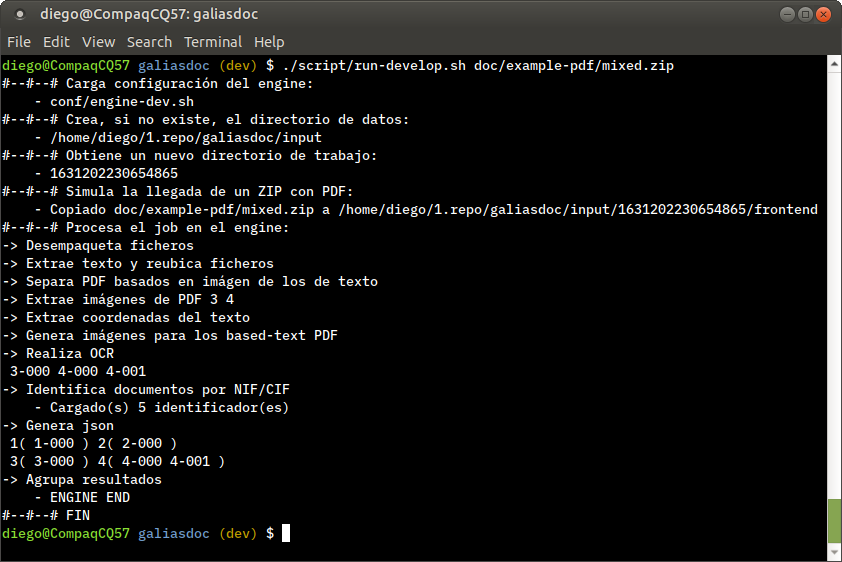
\includegraphics[width=1.0\textwidth]{imaxes/z-adicional/run-develop}
    \caption{Ejecutando manualmente la aplicación}
    \label{fig:ejecucion-manual}
\end{figure}

\section{Visor del formato hOCR}

Existen herramientas para trabajar con el formato hOCR, por ejemplo, las que están disponibles en el repositorio de código del proyecto OCRopus \footnote{\url{https://github.com/ocropus/hocr-tools}}. Pero si lo que se quiere es poder visualizar gráficamente como aplican las líneas y regiones de un hOCR sobre una página en particular, el Pattern Recognition \& Image Analysis (PRImA) Research Lab de la Universidad de Salford mantiene una utilidad para hacer justo esto \cite{prima_tool_page_viewer}. En la imagen \ref{fig:visor-formato-hocr}, el visor muestra las líneas detectadas para una página del proveedor AC. Además de hOCR, la herramienta soporta otros formatos, algunos ya mencionados en la memoria como, PAGE XML, ALTO XML o FineReader XML.

\begin{figure}[hp!]
    \centering
    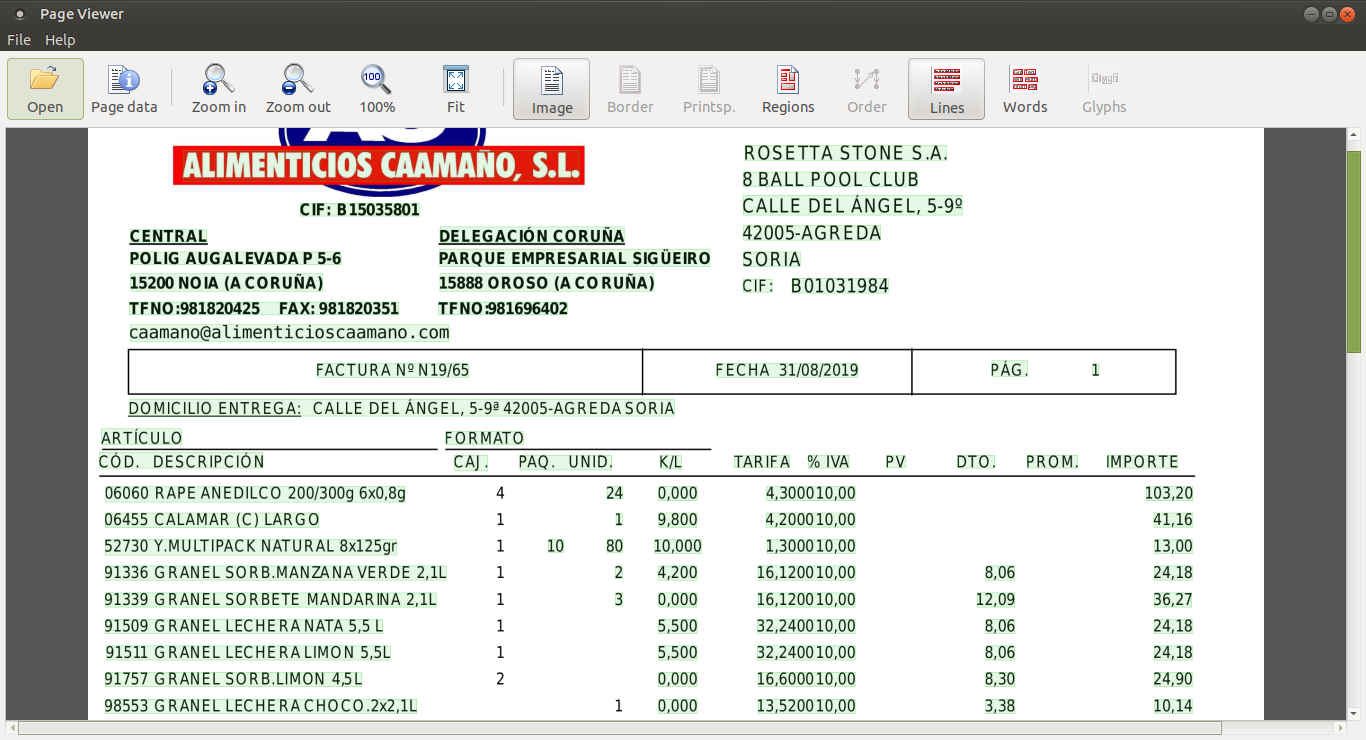
\includegraphics[width=1.0\textwidth]{imaxes/z-adicional/visor-hocr.png}
    \caption{Visor del formato hOCR con un documento de AC}
    \label{fig:visor-formato-hocr}
\end{figure}

\section{Ansible}

% TODO Presentar Ansible y mostrar el script desarrollado

Ansible es una tecnología para automatizar la administración y configuración de ordenadores. Fue creada inicialmente en el año 2012 por Michael DeHaan, hoy en día forma parte del catálogo de productos de Red Hat.

\begin{wrapfigure}{R}{0.3\textwidth}
    \centering
    
\includegraphics[width=0.25\textwidth]{imaxes/e-fundamentos-tecnologicos/logo-ansible.png}
\end{wrapfigure}

Ansible es una tecnología del ámbito de la Gestión de la Configuración. Durante los años 50, el Departamento de Defensa de los Estados Unidos, tenía necesidad de crear una metodología para mantener actualizado el inventario de los recursos materiales disponibles. La Gestión de la Configuración es aquel conjunto de procesos que permiten gestionar los cambios en un sistema, utilizando un método conocido, de tal manera que se mantenga la integridad del sistema a lo largo del tiempo. La manera de lograrlo es manteniendo un registro de los cambios a los que a sido sometido, consiguiendo así conocer cual es el estado actual y como se ha llegado hasta él. Métrica v.3 es un ejemplo de metodología española que incluye la Gestión de la Configuración entre actividades.

Estas ideas se comenzaron a aplicar a los ordenadores para llevar registro tanto del hardware como de los Sistemas Operativos y aplicaciones instaladas. Gracias al avance y aparición de tecnologías como Ansible, en lugar de generar documentos describiendo los estados, se pasa directamente a especificar cuales son los estados deseados y la herramienta realiza los cambios necesarios para asegurar que el estado alcanzado sea el correcto tras la intervención.

Ansible está escrito en Python y su funcionamiento es simple. Para realizar la gestión, conecta a las máquinas mediante el protocolo SSH y aplica los cambios indicados en los ficheros conocidos como Playbooks. Estos ficheros son guiones escritos en lenguaje YAML que indican a Ansible las acciones a acometer. La sintaxis de YAML guarda parecidos con Markdown y es fácil de comprender.

En los Listados \ref{lst:script-ansible-1} y \ref{lst:script-ansible-2} se muestra el Playbook desarrollado para realizar la instalación del software en un servidor remoto.

\noindent\begin{minipage}{.45\textwidth}
	\begin{lstlisting}[language=C,caption={Playbook parte 1},label={lst:script-ansible-1}]{}
---
- name: deploy project to staging
  vars:
    app_dir: solcoerp
    repo_dir: solcoerp-repo
    deploy_dir: deploy
    input_dir: input
  vars_files:
    - svn-credentials.yml
  hosts: backendservers
  remote_user: "{{user}}"
  gather_facts: false
  tasks:
    - name: Remove old deploy directory
      file:
        path: "{{ app_dir }}"
        state: absent
    - name: Check out from repository
      subversion: 
        repo: "{{ repo_url }}"
        dest: "{{ repo_dir }}"
        username: "{{ username }}"
        password: "{{ password }}"
	\end{lstlisting}
\end{minipage}\hfill
\begin{minipage}{.45\textwidth}
	\begin{lstlisting}[language=C,caption={Playbook parte 2},label=lst:script-ansible-2]{}
- name: Call Makefile deploy task
  make:
    chdir: "{{ repo_dir }}"
    target: deploy
- name: Create a root dir for the app 
  file:
    path: "{{ app_dir }}"
    state: directory
- name: Create input directory
  file:
    path: "{{ app_dir  }}/{{ input_dir }}"
    state: directory
- name: Copy deploy dir as app dir 
  copy:
    src: "$HOME/{{ repo_dir }}/{{ deploy_dir }}/"
    dest: "$HOME/{{ app_dir }}/app"
    remote_src: yes 
- name: Remove repo directory
  file:
    path: "{{ repo_dir }}"
    state: absent
	\end{lstlisting}
\end{minipage}


